\chapter{Re-entrant wedges}
\label{ch:re-entrant}

In this chapter,
numerical boundary tracing is applied to re-entrant capillary wedges,
i.e.~wedges with half-angle~$\alpha > \pi/2$.
For simplicity we only consider infinite wedge domains,
for which uniqueness rules out the asymmetric situations observed by
Korevaar~\cite{korevaar-1980-capillary-re-entrant-corner}
and by King~\etal~\cite{king-1999-laplace-young-near-corner}.
We take a numerical solution to
the scaled capillary BVP~(\ref{eq:scaled-laplace-young})
\&~(\ref{eq:scaled-contact-boundary-condition})
in a wedge
and seek rounding curves along which
the contact condition~(\ref{eq:scaled-contact-boundary-condition})
remains satisfied.
Finally, practical results are obtained for the dip-coating problem
of Figure~\ref{fig:dip_coating},
by embracing the sharp corners
that have heretofore been avoided
for the sake of constructing smooth corner roundings.

\section{Numerical wedge solutions}
\label{sec:re-entrant.numerical}

In this section we obtain numerical wedge solutions
to the capillary BVP~(\ref{eq:scaled-laplace-young})
\&~(\ref{eq:scaled-contact-boundary-condition}).
Finite element meshes are constructed in an identical manner
to Section~\ref{sec:moderate.nonlinear.numerical.wedge}.
The domain is taken to be the sector $0 < r < 10$, $-\alpha < \phi < \alpha$
(Figure~\ref{fig:wedge_obtuse-numerical-domain}).
All mesh elements are required to have no more area
than an equilateral triangle of side length~$0.2$,
and we apply the minimalistic refinement strategy
of Section~\ref{sec:moderate.nonlinear.numerical.half-plane}
along the two wedge walls
using a fine length scale of~$0.01$.
For an $\alpha = \SI{135}{\degree}$~wedge,
the resulting mesh consists of around 32000~elements.
The refinement detail near the corner
is shown in Figure~\ref{fig:wedge_obtuse-mesh-detail}.
The full mesh is too large to display here,
but it is very similar to the mesh of Figure~\ref{fig:wedge_acute-mesh-full}.

\begin{figure}
  \begin{minipage}[t]{0.48\textwidth}
    \centredfigurecontent{wedge_obtuse-numerical-domain}{
      Domain for numerical wedge solutions.
    }
  \end{minipage}
  \hfill
  \begin{minipage}[t]{0.48\textwidth}
    \centredfigurecontent[
      width=0.85\textwidth,
      trim=0 {-0.115\textwidth} 0 0,
    ]{%
      wedge_obtuse-mesh-detail%
    }{
      Close-up of finite element mesh
      for an $\alpha = \SI{135}{\degree}$~wedge.
    }
  \end{minipage}
\end{figure}

As before, we obtain numerical solutions in \software{Mathematica}
by specifying the capillary BVP
as the steady-state diffusion problem~(\ref{eq:laplace-young-diffusion})
\&~(\ref{eq:contact-boundary-condition-diffusion}),
with the non-wetting contact condition~%
  (\ref{eq:natural-boundary-condition-diffusion})
applied on the outer arc~$r = 10$
to approximate a vanishing height rise at infinity.
A selected example is shown
in Figure~\ref{fig:wedge_obtuse-solution}.

\begin{figure}
  \centredfigurecontent[width=0.6\textwidth]{wedge_obtuse-solution}{
    Numerical solution
    for~$\alpha = \SI{135}{\degree}$ and~$\gamma = \SI{60}{\degree}$.
  }
\end{figure}

Having precluded asymmetry about~$y = 0$,
the wedge solutions should take on
the locally planar form~(\ref{eq:moderate-wedge-asymptotic-solution})
in the moderate wedge case~$\alpha < \pi/2 + \gamma$;
for the large wedge case~$\alpha \ge \pi/2 + \gamma$,
the corner slope should be unbounded
(with the height remaining bounded).
Table~\ref{tab:re-entrant-wedge-slope}
compares theoretical and computed values of corner slope
for an $\alpha = \SI{135}{\degree}$~wedge.
Unlike the convex wedge case (Table~\ref{tab:convex-wedge-height-slope})
where excellent agreement was observed,
the discrepancy here is rather large,
exceeding~$\SI{10}{\percent}$ in most cases;
moreover we observe a gradual rather than a significant increase
in the computed corner slope
as the contact angle decreases past
the critical angle~$\gamma = \SI{45}{\degree}$.

\begin{table}
  \centering
  \begin{tabular}{
    S[table-format=2, table-space-text-post=\si{\degree}]
    S[table-format=1.4, round-mode=places, round-precision=4]
    S[table-format=2.4, round-mode=places, round-precision=4]
    S[table-format=+1.2, round-mode=places, round-precision=2]
  }
    \toprule
      {$\gamma$}  &
      {\makecell{Theoretical \\ slope}}  &
      {\makecell{Computed \\ slope}}  &
      {\makecell{Relative \\ error}} \\
    \midrule
      30 \si{\degree}  &  {$\infty$}  &   3.52005   &  {N/A} \\
      35 \si{\degree}  &  {$\infty$}  &   2.63412   &  {N/A} \\
      40 \si{\degree}  &  {$\infty$}  &   2.01889   &  {N/A} \\
      45 \si{\degree}  &  {$\infty$}  &   1.57999   &  {N/A} \\
      50 \si{\degree}  &   2.18146    &   1.25446   &  -0.424943 \\
      55 \si{\degree}  &   1.38701    &   1.00256   &  -0.277178 \\
      60 \si{\degree}  &   1.         &   0.799529  &  -0.200471 \\
      65 \si{\degree}  &   0.745469   &   0.629466  &  -0.15561 \\
      70 \si{\degree}  &   0.552637   &   0.481984  &  -0.127846 \\
      75 \si{\degree}  &   0.39332    &   0.349919  &  -0.110345 \\
      80 \si{\degree}  &   0.253333   &   0.228101  &  -0.0995994 \\
      85 \si{\degree}  &   0.124204   &   0.112559  &  -0.0937547 \\
    \bottomrule
  \end{tabular}
  \caption{
    Numerical results for corner slope
    in an $\alpha = \SI{135}{\degree}$~wedge,
    for various contact angles~$\gamma$.
    The critical angle (borderline case) is~$\gamma = \SI{45}{\degree}$.
  }
  \label{tab:re-entrant-wedge-slope}
\end{table}

\begin{figure}
  \centredfigurecontent[width=0.4\textwidth]{%
    wedge_obtuse-mesh-detail-additional-refinement%
  }{%
    Close-up of finite element mesh with additional refinement
    at the ultra-fine length scale~$\ell_\ultra = 0.001$
    applied in the neighbourhood~$r < 0.01$.
  }
\end{figure}

Since boundary tracing relies on
the ability to accurately compute first derivatives
of the wedge solution,
the relatively poor results for the corner slope
are a cause for concern.
Further investigation shows that the computed value of corner slope
is rather sensitive to the level of mesh refinement.
We consider the moderate wedge~%
  $(\alpha, \gamma) = (\SI{135}{\degree}, \SI{60}{\degree})$
and apply localised additional refinement,
using an ultra-fine length scale of~$\ell_\ultra$
in the neighbourhood~$r < 0.01$.
Note that $\ell_\ultra = 0.01$~corresponds roughly
to the existing level of refinement
(Figure~\ref{fig:wedge_obtuse-mesh-detail}),
while $\ell_\ultra < 0.01$~introduces further refinement near the corner
(Figure~\ref{fig:wedge_obtuse-mesh-detail-additional-refinement}).
Although decreasing~$\ell_\ultra$
brings the computed corner slope closer
to the the theoretical value of unity
(Table~\ref{tab:re-entrant-wedge-slope-additional-refinement}),
even an impractically large number of mesh elements
achieves only an accuracy of~$\SI{6}{\percent}$.
However, from Figure~\ref{fig:wedge_obtuse-moderate-additional-refinement}
we see that the solution slope only depends significantly on~$\ell_\ultra$
in the immediate vicinity of the corner, $r < 0.003$;
outside this tiny neighbourhood
the computed slope is indeed consistent.
Therefore, provided we interpret near-corner results with caution,
the numerical wedge solutions obtained
using the existing level of mesh refinement
will be adequate for the purposes of boundary tracing;
the additional near-corner refinement is not necessary.
We are also reassured by the fact that,
unlike corner slope,
the same value of corner height is consistently obtained,
both with and without the additional refinement.

\begin{table}
  \centering
  \begin{tabular}{
    S[table-format=1.4]
    S[table-format=6]
    S[table-format=1.4, round-mode=places, round-precision=4]
    S[table-format=+1.2, round-mode=places, round-precision=2]
  }
    \toprule
      {$\ell_\ultra$}  &
      {\makecell{Mesh \\ elements}}  &
      {\makecell{Computed \\ slope}}  &
      {\makecell{Relative \\ error}} \\
    \midrule
      0.0001  &  121071  &  0.941074  &  -0.058926 \\
      0.0002  &   55171  &  0.930714  &  -0.0692859 \\
      0.0005  &   36147  &  0.915463  &  -0.0845373 \\
      0.001   &   33361  &  0.899529  &  -0.100471 \\
      0.01    &   32230  &  0.823078  &  -0.176922 \\
    \bottomrule
  \end{tabular}
  \caption{
    Numerical results for corner slope
    in an $(\alpha, \gamma) = (\SI{135}{\degree}, \SI{60}{\degree})$~wedge,
    with additional refinement
    at various ultra-fine length scales~$\ell_\ultra$
    applied in the neighbourhood~$r < 0.01$.
  }
  \label{tab:re-entrant-wedge-slope-additional-refinement}
\end{table}

\begin{figure}
  \newcommand*{\subfigurewidth}{0.45\textwidth}
  \centering
  $\ell_\ultra$
  \includegraphics[width=\textwidth, trim=0 10 0 10]{%
    wedge_obtuse-moderate-slope-additional-refinement-legend%
  }
  \hspace*{\fill}
  \begin{subfigure}[t]{\subfigurewidth}
    \includegraphics[width=\textwidth]{%
      wedge_obtuse-moderate-slope-additional-refinement-symmetry%
    }
    \includegraphics[width=\textwidth]{%
      wedge_obtuse-moderate-height-additional-refinement-symmetry%
    }
    \caption{%
      Along line of symmetry~$\phi = 0$
    }
    \label{fig:wedge_obtuse-moderate-additional-refinement-symmetry}
  \end{subfigure}
    \hfill
  \begin{subfigure}[t]{\subfigurewidth}
    \includegraphics[width=\textwidth]{%
      wedge_obtuse-moderate-slope-additional-refinement-wall%
    }
    \includegraphics[width=\textwidth]{%
      wedge_obtuse-moderate-height-additional-refinement-wall%
    }
    \caption{%
      Along wedge wall~$\phi = \alpha$
    }
    \label{fig:wedge_obtuse-moderate-additional-refinement-wall}
  \end{subfigure}
  \hspace*{\fill}
  \caption{
    Computed slope and height near the corner
    for the moderate re-entrant wedge~%
      $(\alpha, \gamma) = (\SI{135}{\degree}, \SI{60}{\degree})$,
    with additional refinement
    at various ultra-fine length scales~$\ell_\ultra$
    applied in the neighbourhood~$r < 0.01$.
    The theoretical slope in the corner~($r = 0$) is unity.
  }
  \label{fig:wedge_obtuse-moderate-additional-refinement}
\end{figure}

Similar results are observed
for large wedge angles~$\alpha \ge \pi/2 + \gamma$,
where the theoretical corner slope is unbounded
but the height remains bounded.
In the specific case of~%
  $(\alpha, \gamma) = (\SI{135}{\degree}, \SI{30}{\degree})$
shown in Figure~\ref{fig:wedge_obtuse-large-additional-refinement},
we observe that any dependence of the solution slope
on the refinement scale~$\ell_\ultra$
is confined to the minuscule neighbourhood~$r < 0.002$.
Again we find the solution height to be
completely insensitive to~$\ell_\ultra$,
even at the corner~$r = 0$ itself.

\begin{figure}
  \newcommand*{\subfigurewidth}{0.45\textwidth}
  \centering
  $\ell_\ultra$
  \includegraphics[width=\textwidth, trim=0 10 0 10]{%
    wedge_obtuse-moderate-slope-additional-refinement-legend%
  }
  \hspace*{\fill}
  \begin{subfigure}[t]{\subfigurewidth}
    \includegraphics[width=\textwidth]{%
      wedge_obtuse-large-slope-additional-refinement-symmetry%
    }
    \includegraphics[width=\textwidth]{%
      wedge_obtuse-large-height-additional-refinement-symmetry%
    }
    \caption{%
      Along line of symmetry~$\phi = 0$
    }
    \label{fig:wedge_obtuse-large-additional-refinement-symmetry}
  \end{subfigure}
    \hfill
  \begin{subfigure}[t]{\subfigurewidth}
    \includegraphics[width=\textwidth]{%
      wedge_obtuse-large-slope-additional-refinement-wall%
    }
    \includegraphics[width=\textwidth]{%
      wedge_obtuse-large-height-additional-refinement-wall%
    }
    \caption{%
      Along wedge wall~$\phi = \alpha$
    }
    \label{fig:wedge_obtuse-large-additional-refinement-wall}
  \end{subfigure}
  \hspace*{\fill}
  \caption{
    Computed slope and height near the corner
    for the large wedge~%
      $(\alpha, \gamma) = (\SI{135}{\degree}, \SI{30}{\degree})$,
    with additional refinement
    at various ultra-fine length scales~$\ell_\ultra$
    applied in the neighbourhood~$r < 0.01$.
    The theoretical slope in the corner~($r = 0$) is infinite.
  }
  \label{fig:wedge_obtuse-large-additional-refinement}
\end{figure}

\section{Corner rounding}
\label{sec:re-entrant.rounding}

In this section,
we take the numerical wedge solutions that have just been obtained
and perform boundary tracing
to seek roundings of the wedge corner.

\subsection{Boundary tracing}
\label{sec:re-entrant.rounding.tracing}

First we consider the default case,
where the contact angle for boundary tracing
is the same as the contact angle~$\gamma$
for the known numerical solution~$T$.

Proceeding as in Section~\ref{sec:moderate.nonlinear.tracing},
the contact condition~(\ref{eq:scaled-contact-boundary-condition})
is rewritten as
\begin{important}{equation}
  \normalvec \dotp \del T = \cos\gamma \sqrt{1 + (\del T)^2},
  \label{eq:re-entrant-flux-boundary-condition}
\end{important}
and we again have flux function
\begin{equation}
  F \ideq \cos\gamma \sqrt{1 + (\del T)^2},
  \label{eq:re-entrant-flux-function}
\end{equation}
viability function
\begin{equation}
  \Phi \ideq \sin^2\gamma \, (\del T)^2 - \cos^2\gamma,
  \label{eq:re-entrant-viability-function}
\end{equation}
and viable domain
\begin{equation}
  \norm{\del T} \ge \cot\gamma.
  \label{eq:re-entrant-viable-domain}
\end{equation}
The non-viable domain is shown
in Figure~\ref{fig:wedge_obtuse-viable},
with a larger-scale version
in Figure~\ref{fig:wedge_obtuse-viable-larger-scale}.
Away from the corner but near the walls,
the wedge solution may be approximated by the half-plane solution
with contact angle~$\gamma$
(and hence slope~$\cot\gamma$)
along the wall;
therefore the terminal curve
\begin{equation}
  \norm{\del T} = \cot\gamma
  \label{eq:re-entrant-terminal-curve}
\end{equation}
asymptotes to the wedges walls as one travels away from the wedge corner.
The viable domain lies to the left of the terminal curve
and hugs the wedge walls.

\begin{figure}
  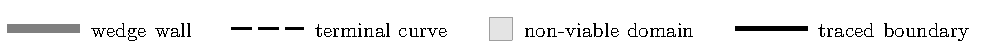
\includegraphics[width=\textwidth, trim=0 -10 0 0]{helmholtz-legend}
  \begin{minipage}[t]{0.5\textwidth}
    \centredfigurecontent[width=0.7\textwidth]{%
      wedge_obtuse-viable%
    }{
      Non-viable domain~$\Phi < 0$
      for~$\alpha = \SI{135}{\degree}$ and~$\gamma = \SI{60}{\degree}$.
    }
  \end{minipage}
  \begin{minipage}[t]{0.5\textwidth}
    \centredfigurecontent[width=0.7\textwidth]{%
      wedge_obtuse-traced-boundaries%
    }{
      Traced boundaries
      for~$\alpha = \SI{135}{\degree}$ and~$\gamma = \SI{60}{\degree}$,
      obtained by integrating~%
        (\ref{eq:re-entrant-tracing-ode-arc-length-parametrisation-x})
      \&~%
        (\ref{eq:re-entrant-tracing-ode-arc-length-parametrisation-y}).
    }
  \end{minipage}
\end{figure}

\begin{figure}
  \centredfigurecontent[width=0.36\textwidth]{%
    wedge_obtuse-viable-larger-scale%
  }{
    Non-viable domain~$\Phi < 0$ on a larger scale.
  }
\end{figure}

Working in Cartesian coordinates as before,
we have the derivatives
\begin{align}
  P &\ideq \pder{T}{x},
    \label{eq:re-entrant-gradient-x-component} \\[\tallspace]
  Q &\ideq \pder{T}{y}.
    \label{eq:re-entrant-gradient-y-component}
\end{align}
Again the boundary tracing system of ODEs for arc-length parametrisation
reduces to
\begin{important}{align}
  \tder{x}{s} &= \frac{-Q F \pm P \sqrt{\Phi}}{(\del T)^2},
    \label{eq:re-entrant-tracing-ode-arc-length-parametrisation-x}
    \\[\tallspace]
  \tder{y}{s} &= \frac{+P F \pm Q \sqrt{\Phi}}{(\del T)^2},
    \label{eq:re-entrant-tracing-ode-arc-length-parametrisation-y}
\end{important}
and we obtain traced boundaries
as in Figure~\ref{fig:wedge_obtuse-traced-boundaries}
by performing numerical integration
from starting points within the viable domain.

As in the convex-wedge case,
the original wedge walls~$\phi = \pm\alpha$
are themselves traced boundaries.
It is reassuring that the walls can be recovered
by starting the integration at precisely~$(x, y) = (0, 0)$,
as this suggests that the results of boundary tracing near the corner
are valid
despite the earlier concerns (Section~\ref{sec:re-entrant.numerical})
regarding the computed value of slope in the corner.
Relative to the convex-wedge case,
a swapping of the two branches has occurred;
the top wall~$\phi = +\alpha$ now belongs to the lower branch
of~(\ref{eq:re-entrant-tracing-ode-arc-length-parametrisation-x})
\&~(\ref{eq:re-entrant-tracing-ode-arc-length-parametrisation-y}),
rather than the upper branch.
The swapping of branches at~$\alpha = \pi/2$ may be seen
by substituting the locally planar form~%
  (\ref{eq:moderate-asymptotic-solution});
without assuming either a convex or a re-entrant wedge,
the boundary tracing system of ODEs reduces to
\begin{align}
  \tder{x}{s} &\asy \mp \abs{\cos\alpha},
    \label{eq:planar-asymptotic-tracing-ode-arc-length-parametrisation-x}
    \\[\tallspace]
  \tder{y}{s} &= -\sin\alpha,
    \label{eq:planar-asymptotic-tracing-ode-arc-length-parametrisation-y}
\end{align}
so that
\begin{equation}
  \tder{y}{x} \asy \frac{\pm\sin\alpha}{\abs{\cos\alpha}} =
    \begin{cases}
      \pm\tan\alpha, &\text{$\alpha < \pi/2$ (convex)} \\
      \mp\tan\alpha, &\text{$\alpha > \pi/2$ (re-entrant)}
    \end{cases}
  \label{eq:planar-asymptotic-tracing-ode-coordinate-parametrisation-y}
\end{equation}
for traced boundaries near the corner.

\begin{figure}
  \centredfigurecontent[width=0.63\textwidth]{%
    wedge_obtuse-terminal-points%
  }{
    $T$-contours which intersect the terminal curve~$\Phi = 0$.
  }
\end{figure}

We return now to
Figure~\ref{fig:wedge_obtuse-traced-boundaries}
and attempt to construct a rounding of the corner
by patching together the traced boundaries.
As in Section~\ref{sec:moderate.nonlinear.tracing},
corners are inevitably formed \emph{strictly} within the viable domain;
therefore any smooth patching together must necessarily occur
along the terminal curve~(\ref{eq:re-entrant-terminal-curve}).
Inspecting Figure~\ref{fig:wedge_obtuse-terminal-points},
we see that almost all points along the terminal curve are ordinary,
for which the two local traced boundaries form a cusp
with inconsistent boundary orientation.
As before, the only exception is
a single critical terminal point
along the line of symmetry~$y = 0$,
explicitly~$(x, y) = (x_0, 0)$,
where $x = x_0$~is the unique solution to
\begin{equation}
  \eval*{-\pder{T}{x}}_{y=0} = \cot\gamma.
  \label{eq:re-entrant-critical-terminal-point}
\end{equation}
Unlike the convex wedge case,
the local $T$-contour lies toward
the non-viable side of the the terminal curve;
the critical terminal point~$(x_0, 0)$ is therefore of elliptic type,
and there are no smooth traced boundaries passing through it.
Thus we cannot construct a rounding of the corner.

\begin{figure}
  \newcommand*{\subfigurewidth}{0.45\textwidth}
  \newcommand*{\subfiguregraphicswidth}{0.65\textwidth}
  \centering
  \hspace*{\fill}
  \begin{subfigure}[t]{\subfigurewidth}
    \centredfigurecontent[width=\subfiguregraphicswidth]{%
      wedge_obtuse-traced-boundaries-upper-branch%
    }{%
      Upper branch
    }
  \end{subfigure}
    \hfill
  \begin{subfigure}[t]{\subfigurewidth}
    \centredfigurecontent[width=\subfiguregraphicswidth]{%
      wedge_obtuse-traced-boundaries-lower-branch%
    }{%
      Lower branch
    }
  \end{subfigure}
  \hspace*{\fill}
  \caption{
    Traced boundaries segregated by branch.
  }
  \label{fig:wedge_obtuse-traced-boundaries-branches}
\end{figure}

In fact there are no new domains at all,
even with sharp corners,
that can be constructed from the traced boundaries
of Figure~\ref{fig:wedge_obtuse-traced-boundaries}.
Let us briefly view the traced boundaries
as trajectories of a dynamical system,
with direction of travel as shown in
Figure~\ref{fig:wedge_obtuse-traced-boundaries-branches}.
Recall that in the case of a convex wedge,
the original wedge walls were stable manifolds of their respective branches,
as confirmed by the perturbation analysis
of Section~\ref{sec:moderate.nonlinear.approach}
(which culminated in the estimate~%
  (\ref{eq:moderate-perturbation-near-wall-approach})
for the rate at which traced boundaries approached the wall).
For a re-entrant wedge we find the opposite;
indeed a similar perturbation analysis
(again using wall coordinates~$\xi$ and~$\eta$)
yields
\begin{equation}
  \tder{\vd\xi}{\eta} \asy
    \squarebr*{
      +\frac{h}{\sin\gamma} \cdot \roundbr*{\pder{T}{\eta}}^{-1}
    }_{\xi=0}
      \cdot \vd\xi,
  \label{eq:re-entrant-perturbation-near-wall-repulsion}
\end{equation}
with the numerical evidence indicating that
$\pd T / {\pd\eta}$~is positive along the wall
(i.e.~the height rise along the wall increases
as one moves away from the corner).
The wedge walls are therefore unstable;
the traced boundaries are repelled from the walls,
eventually colliding with the terminal curve and terminating.
Thus, the only traced boundaries which extend to infinity
are the original wedge walls themselves,
and no new domains can be constructed.

\subsection{Different contact angle}
\label{sec:re-entrant.rounding.different}

The bleak outlook persists
even when a different tracing contact angle~$\gamma_\tr$ is used
to the contact angle~$\gamma$ of the known solution.
As in Section~\ref{sec:moderate.multiple.different},
we replace the contact condition~(\ref{eq:re-entrant-flux-boundary-condition})
with the more general~%
  (\ref{eq:moderate-flux-boundary-condition-different-angle}),
i.e.
\begin{important}{equation}
  \normalvec \dotp \del T (x, y; \alpha, \gamma) =
    \cos\gamma_\tr
    \sqrt{1 + \squarebr[\bulkysize]{\del T (x, y; \alpha, \gamma)}^2},
  \label{eq:re-entrant-flux-boundary-condition-different-angle}
\end{important}
leading to flux function~(\ref{eq:moderate-flux-function-different-angle}),
viability function~(\ref{eq:moderate-viability-function-different-angle}),
and viable domain~(\ref{eq:moderate-viable-domain-different-angle}).

\begin{figure}
  \newcommand*{\subfigurewidth}{0.45\textwidth}
  \newcommand*{\subfiguregraphicsheight}{1.4\textwidth}
  \centering
  \includegraphics[width=\textwidth, trim=0 -5 0 0]{%
    wedge_acute-traced-boundaries-different-angle-legend%
  }
  \hspace*{\fill}
  \begin{subfigure}[t]{\subfigurewidth}
    \centredfigurecontent[width=!, height=\subfiguregraphicsheight]{%
      wedge_obtuse-traced-boundaries-different-angle-less%
    }{%
      $\gamma_\tr = \SI{58}{\degree} < \gamma$
    }
  \end{subfigure}
    \hfill
  \begin{subfigure}[t]{\subfigurewidth}
    \centredfigurecontent[width=!, height=\subfiguregraphicsheight]{%
      wedge_obtuse-traced-boundaries-different-angle-more%
    }{%
      $\gamma_\tr = \SI{63}{\degree} > \gamma$
    }
  \end{subfigure}
  \hspace*{\fill}
  \caption{
    Traced boundaries for~$\alpha = \SI{135}{\degree}$,
    $\gamma = \SI{60}{\degree}$, and~$\gamma_\tr \ne \gamma$,
    obtained by integrating~%
      (\ref{eq:re-entrant-tracing-ode-arc-length-parametrisation-x})
    \&~%
      (\ref{eq:re-entrant-tracing-ode-arc-length-parametrisation-y}).
  }
  \label{fig:wedge_obtuse-traced-boundaries-different-angle}
\end{figure}

For~$\gamma_\tr < \gamma$
(Figure~\ref{fig:wedge_obtuse-traced-boundaries-different-angle-less}),
we again have a viable domain
that does not extend to infinity,
and a rounding of the corner cannot be produced
from the traced boundaries.

For~$\gamma_\tr > \gamma$
(Figure~\ref{fig:wedge_obtuse-traced-boundaries-different-angle-more}),
the viable domain does extend to infinity,
and as in Section~\ref{sec:moderate.multiple.different},
the avoidance of corners leads us to
a lone critical terminal point~$(x_0, 0)$
at the intersection between the terminal curve
and the line of symmetry~$y = 0$,
with $x = x_0$~being the unique solution to
\begin{equation}
  \eval*{-\pder{T}{x}}_{y=0} = \cot\gamma_\tr.
  \label{eq:re-entrant-critical-terminal-point-different-angle}
\end{equation}
Unfortunately $(x_0, 0)$~is of elliptic type;
the local $T$-contour lies toward the non-viable side of the terminal curve
(qualitatively no different to the $\gamma_\tr = \gamma$~case,
Figure~\ref{fig:wedge_obtuse-terminal-points}),
so we cannot construct a rounding of the corner.

\begin{figure}
  \newcommand*{\subfigurewidth}{0.45\textwidth}
  \newcommand*{\subfiguregraphicswidth}{0.75\textwidth}
  \centering
  \hspace*{\fill}
  \begin{subfigure}[t]{\subfigurewidth}
    \centredfigurecontent[width=\subfiguregraphicswidth]{%
      wedge_obtuse-traced-boundaries-different-angle-upper-branch%
    }{%
      Upper branch
    }
  \end{subfigure}
    \hfill
  \begin{subfigure}[t]{\subfigurewidth}
    \centredfigurecontent[width=\subfiguregraphicswidth]{%
      wedge_obtuse-traced-boundaries-different-angle-lower-branch%
    }{%
      Lower branch
    }
  \end{subfigure}
  \hspace*{\fill}
  \caption{
    Traced boundaries~\figurestyle{grey} for~$\gamma_\tr > \gamma$.
    For each branch, the black trajectory extends to infinity
    but is unstable with respect to the direction of travel shown.
  }
  \label{fig:wedge_obtuse-traced-boundaries-different-angle-branches}
\end{figure}

While the situation appears hopeless,
useful results may yet be gleaned
by relaxing the absolute requirement of smoothness.
In Section~\ref{sec:re-entrant.rounding.tracing},
we saw for~$\gamma_\tr = \gamma$ that the original wedge walls were
the only traced boundaries extending to infinity,
and that they were unstable with respect to the direction of travel
in Figure~\ref{fig:wedge_obtuse-traced-boundaries-branches}.
In the present situation~$\gamma_\tr > \gamma$,
each branch again has an unstable manifold extending to infinity
(Figure~\ref{fig:wedge_obtuse-traced-boundaries-different-angle-branches}),
but these manifolds are not the walls
(nor do they approach them).
By the same reasoning as in Section~\ref{sec:moderate.multiple.different},
the two manifolds instead approach
a new wedge~$\xi = d (\gamma, \gamma_\tr)$
offset from the walls~$\xi = 0$;
see~(\ref{eq:moderate-offset-wedge})
and~(\ref{eq:moderate-offset-distance}).
In practice, the two manifolds are computed
by travelling in the opposite direction,
i.e.~towards the line of symmetry~$y = 0$
(Figure~\ref{fig:wedge_obtuse-pseudo-rounding-construction-direction}),
so that we have stability rather than instability.
The two trajectories eventually intersect,
and by symmetry this occurs at a point~$(x_\corn, 0)$.
By trimming the excess and patching the two boundaries together
(Figure~\ref{fig:wedge_obtuse-pseudo-rounding-construction-corner}),
we obtain a curve which we shall call a \emph{pseudo-rounding} of the corner;
while it is not a perfect rounding
due to the corner formed at~$(x_\corn, 0)$,
the corner angle deviates in most cases
by only a few degrees from a straight angle,
and for practical purposes
the corner may be regarded as a rounded one.

\begin{figure}
  \newcommand*{\subfigurewidth}{0.45\textwidth}
  \newcommand*{\subfiguregraphicsheight}{1.15\textwidth}
  \centering
  \hspace*{\fill}
  \begin{subfigure}[t]{\subfigurewidth}
    \centredfigurecontent[width=!, height=\subfiguregraphicsheight]{%
      wedge_obtuse-pseudo-rounding-construction-direction%
    }{%
      Start far from the corner
      at the offset distance~$\xi = d (\gamma, \gamma_\tr)$
      from the wall, and integrate towards the corner
    }
  \end{subfigure}
    \hfill
  \begin{subfigure}[t]{\subfigurewidth}
    \centredfigurecontent[width=!, height=\subfiguregraphicsheight]{%
      wedge_obtuse-pseudo-rounding-construction-corner%
    }{%
      Patch the traced boundaries together
      by trimming and joining at~$(x_\corn, 0)$
    }
  \end{subfigure}
  \hspace*{\fill}
  \caption{
    Construction of a pseudo-rounding for~$\gamma_\tr > \gamma$.
  }
  \label{fig:wedge_obtuse-pseudo-rounding-construction}
\end{figure}

Thus, given a single numerical wedge solution~$T (x, y; \alpha, \gamma)$
in a re-entrant wedge,
a one-parameter family of pseudo-roundings may be generated
using boundary tracing,
corresponding to different contact angles~$\gamma_\tr > \gamma$
(Figure~\ref{fig:wedge_obtuse-pseudo-roundings}).
In cases where~$\gamma_\tr > \gamma + \SI{10}{\degree}$,
the corner~$(x_\corn, 0)$ lies very near
to the critical terminal point~$(x_0, 0)$,
and the pseudo-rounding is practically indistinguishable
from a perfectly smooth rounding.

\begin{figure}
  \centredfigurecontent[width=0.4\textwidth]{%
    wedge_obtuse-pseudo-roundings%
  }{%
    One-parameter family of pseudo-roundings for~$\gamma_\tr > \gamma$,
    all obtained from the wedge solution
    for~$\alpha = \SI{135}{\degree}$ and~$\gamma = \SI{60}{\degree}$.
    From left to right:
    $\gamma_\tr =
      \SI{65}{\degree}, \SI{70}{\degree}, \dots, \SI{85}{\degree}$.
  }
\end{figure}

As in Section~\ref{sec:moderate.multiple.effect},
we observe that in physical problems,
it is the contact angle~$\gamma_\tr$ which is given,
as opposed to~$\gamma$;
therefore we group the pseudo-roundings by~$\gamma_\tr$
rather than~$\gamma$.
We then apply the horizontal offset~(\ref{eq:moderate-horizontal-translation})
so that the curves can be compared as pseudo-roundings
of the same wedge~$y = \pm \offset{x} \tan\alpha$
(Figure~\ref{fig:wedge_obtuse-pseudo-roundings-offset}).
Unlike the convex wedge case,
bulging problems do not occur for any~$\alpha$.
While the pseudo-roundings here are not as close to circular arcs
as the smooth roundings of Section~\ref{sec:moderate.multiple.effect},
they still provide some information
on the effect of corner rounding on height rise.
By evaluating the relevant known solution
along each pseudo-rounding,
we may obtain a family of height-rise profiles
as shown in Figure~\ref{fig:wedge_obtuse-height-rise-profiles}.

\begin{figure}
  \centredfigurecontent[width=0.38\textwidth]{%
    wedge_obtuse-pseudo-roundings-offset%
  }{%
    Pseudo-roundings for~$\gamma < \gamma_\tr$
    in $(\offset{x}, y)$~coordinates,
    all corresponding to the physically prescribed contact angle~%
    $\gamma_\tr = \SI{60}{\degree}$.
    From left to right:
    $\gamma = \SI{10}{\degree}, \SI{20}{\degree}, \dots, \SI{50}{\degree}$.
  }
\end{figure}

\begin{figure}
  \centredfigurecontent[width=0.6\textwidth]{%
    wedge_obtuse-height-rise-profiles%
  }{
    Height-rise profiles (parametrised by arc length)
    for~$\alpha = \SI{135}{\degree}$ and~$\gamma_\tr = \SI{60}{\degree}$,
    along the original wedge~\figurestyle{grey},
    and along the constructed psuedo-roundings of the corner
    for~$\gamma = \SI{10}{\degree}, \SI{40}{\degree}$~%
      \figurestyle{solid black, top to bottom along~$s = 0$}.
    The wall height~(\ref{eq:half-plane-height-different-angle})~%
      \figurestyle{dotted}
    is shown for reference.
    Note the exaggerated vertical scale.
  }
\end{figure}

\section{Dip-coating}
\label{sec:re-entrant.dip-coating}

While corner rounding reduces the amount of arching near a corner
(as we have just seen in Figure~\ref{fig:wedge_obtuse-height-rise-profiles}),
it is not able to completely eliminate it.
In the practical dip-coating problem of
Figure~\ref{fig:dip_coating},
the ideal coating profile is completely flat,
and in this section we utilise a different approach
in order to achieve this goal.
Indeed our avoidance of joinings with sharp corners
(amidst the search for smooth rounding curves)
has been severely restrictive
on the variety of shapes that can be produced by boundary tracing.
Here we change tack and use to our advantage
the corners that we have hitherto avoided.

\subsection{Roughness}
\label{sec:re-entrant.dip-coating.roughness}

\begin{figure}
  \newcommand*{\subfigurewidth}{0.45\textwidth}
  \newcommand*{\subfiguregraphicswidth}{0.9\textwidth}
  \centering
  \hspace*{\fill}
  \begin{subfigure}[t]{\subfigurewidth}
    \centredfigurecontent[width=\subfiguregraphicswidth]{%
      wedge_obtuse-traced-boundaries-approximation-contour%
    }{%
      $T$-contour~(\ref{eq:re-entrant-tracing-contour})~\figurestyle{dotted}
    }
  \end{subfigure}
    \hfill
  \begin{subfigure}[t]{\subfigurewidth}
    \centredfigurecontent[width=\subfiguregraphicswidth]{%
      wedge_obtuse-traced-boundaries-approximation-serrated%
    }{%
      Approximating serrated path~\figurestyle{thick black}
    }
  \end{subfigure}
  \hspace*{\fill}
  \caption{
    Approximation of a $T$-contour
    by patching together traced boundaries~\figurestyle{grey}
    for~$\alpha = \SI{135}{\degree}$, $\gamma = \SI{20}{\degree}$,
    and~$\gamma_\tr = \SI{55}{\degree}$.
  }
  \label{fig:wedge_obtuse-traced-boundaries-approximation}
\end{figure}

Consider Figure~\ref{fig:wedge_obtuse-traced-boundaries-approximation-contour},
which shows the two branches of traced boundaries
for a tracing contact angle of~$\gamma_\tr$
(greater than the contact angle~$\gamma$ of the known solution~$T$),
along with the $T$-contour
\begin{equation}
  T = h_\tr,
  \label{eq:re-entrant-tracing-contour}
\end{equation}
where $h_\tr$~is the half-plane wall height~%
  (\ref{eq:half-plane-height-different-angle})
for the contact angle~$\gamma_\tr$.
We assume that $\gamma_\tr$~is large enough
that the $T$-contour steers completely clear of the wedge corner.
Like the pseudo-roundings of Section~\ref{sec:re-entrant.rounding.different},
the $T$-contour~(\ref{eq:re-entrant-tracing-contour})
approaches the offset wedge~$\xi = d (\gamma, \gamma_\tr)$
as one travels away from the line of symmetry~$y = 0$.
It would be nice to have the $T$-contour be a rounding of the corner
(achieving a completely uniform height rise of~$h_\tr$),
but of course the $T$-contour is not a traced boundary.
However, we observe that the $T$-contour may be approximated
by a serrated path made from traced boundary portions
as shown in
Figure~\ref{fig:wedge_obtuse-traced-boundaries-approximation-serrated}.
Taking the region to the right of the path as interior,
we obtain a new domain
for which the height-rise profile is approximately uniform
with height~$h_\tr$;
the finer the serrations,
the closer the profile to being completely level.

Physically, the serrated path
may be thought of as a roughened version
of the $T$-contour~(\ref{eq:re-entrant-tracing-contour}).
The use of small-scale indentations
to model roughness in a capillary context
is not without precedent.
Pioneering work
by Wenzel~\cite{wenzel-1936-resistance-solid-surfaces-wetting}
noted that a rough surface has a greater surface area
than its perfectly smooth counterpart,
so that the effective contact angle and the true contact angle
have a cosine ratio equal to
\begin{equation}
  \textq{roughness factor} =
    \frac{\textq{actual surface area}}{\textq{smooth surface area}}.
  \label{eq:wenzel-roughness}
\end{equation}
(More general models are possible which account for
porosity~\cite{cassie-1944-wettability-porous-surfaces}
and contact angle hysteresis~\cite{
  cox-1983-spreading-liquid-rough-surface,
  johnson-1964-contact-angle-hysteresis
};
these will not be considered here.)
Anderson~\etal~\cite{anderson-2006-exact-solutions-laplace-young}
patched together traced boundaries
arising from the known half-plane solution
to obtain a multitude of walls with indentations
(Figure~\ref{fig:half_plane-traced-boundaries}).
Anderson~\cite[Section~6.4]{anderson-2002-thesis-boundary-tracing-pdes}
obtained Wenzel's cosine result independently%
\footnote{
  Wenzel's derivation was for a liquid drop resting on a horizontal plate,
  while Anderson's derivation was for liquid against a vertical wall;
  both lead to the same result for the effective contact angle.
}
and provided some numerical verification
in the case of sinusoidal indentations.

\begin{figure}
  \centredfigurecontent[width=0.9\textwidth]{%
    capillary-serrated-approximation-geometry%
  }{
    Local geometry of the approximation of a $T$-contour
    with a serrated traced boundary path.
  }
\end{figure}

We repeat here the derivation of
Anderson~\cite[Section~6.4.2]{anderson-2002-thesis-boundary-tracing-pdes},
but adapted to the current context,
in which we are approximating
the~$T$-contour~(\ref{eq:re-entrant-tracing-contour})
with a serrated path of traced boundaries
as in Figure~\ref{fig:wedge_obtuse-traced-boundaries-approximation-serrated}.
Suppose the serrations are small enough
that the $T$-contour and the serrations themselves
may be regarded as straight
(Figure~\ref{fig:capillary-serrated-approximation-geometry}).
Since the serrated path is constructed from traced boundaries
with a tracing contact angle of~$\gamma_\tr$,
we have
\begin{equation}
  \normalvec \dotp \frac{\del T}{\sqrt{1 + (\del T)^2}} = \cos\gamma_\tr
  \label{eq:re-entrant-contact-boundary-condition-serrated}
\end{equation}
along the serrated path.
Now suppose that the known solution~$T$ can also be realised
by replacing the serrated path with the $T$-contour
having an effective contact angle of~$\gamma_\eff$.
Writing~$\normalvec_\eff$ for the normal to the $T$-contour,
we have
\begin{equation}
  \normalvec_\eff \dotp \frac{\del T}{\sqrt{1 + (\del T)^2}} = \cos\gamma_\eff
  \label{eq:re-entrant-contact-boundary-condition-contour}
\end{equation}
along the $T$-contour.
With $\theta$~denoting the angle between~$\normalvec$ and~$\del T$,%
\footnote{
  See the geometric interpretation~(\ref{eq:flux-boundary-condition-cosine})
  of the generic flux boundary condition~(\ref{eq:flux-boundary-condition}).
}
(\ref{eq:re-entrant-contact-boundary-condition-serrated}) becomes
\begin{equation}
  \frac{\norm{\del T} \cos\theta}{\sqrt{1 + (\del T)^2}} = \cos\gamma_\tr,
  \label{eq:re-entrant-contact-boundary-condition-serrated-simplified}
\end{equation}
and since $\normalvec_\eff$~is parallel to~$\del T$,
(\ref{eq:re-entrant-contact-boundary-condition-contour}) becomes
\begin{equation}
  \frac{\norm{\del T}}{\sqrt{1 + (\del T)^2}} = \cos\gamma_\eff.
  \label{eq:re-entrant-contact-boundary-condition-contour-simplified}
\end{equation}
Now from the geometry
of Figure~\ref{fig:capillary-serrated-approximation-geometry},
we see that
\begin{equation}
  \frac{\textq{serrated path length}}{\textq{contour path length}}
   = \frac{1}{\cos\theta},
   \label{eq:path-length-ratio}
\end{equation}
and since both boundaries represent vertical walls,
this ratio is precisely Wenzel's roughness factor~(\ref{eq:wenzel-roughness}).
Denoting the roughness factor by~$\rho$,
and using~(\ref{eq:re-entrant-contact-boundary-condition-serrated-simplified})
and~(\ref{eq:re-entrant-contact-boundary-condition-contour-simplified}),
we therefore have
\begin{important}{equation}
  \rho = \frac{1}{\cos\theta} = \frac{\cos\gamma_\eff}{\cos\gamma_\tr}
  \label{eq:roughness-cosine-ratio}
\end{important}
relating the roughness factor~$\rho$,
the true contact angle~$\gamma_\tr$ along the serrated boundary,
and the effective contact angle~$\gamma_\eff$
along the $T$-contour~(\ref{eq:re-entrant-tracing-contour}).
This completes the derivation.

Note that the roughness factor is always greater than or equal to unity;
a perfectly smooth boundary has~$\rho = 1$,
a rough boundary has~$\rho > 1$,
and a fractal boundary has~$\rho = \infty$.
Thus, for a true contact angle of~$\gamma_\tr$ which is acute,
roughness reduces the effective value of contact angle to
\begin{equation}
  \gamma_\eff = \cos^{-1} \roundbr*{\rho \cos\gamma_\tr}.
  \label{eq:effective-contact-angle}
\end{equation}

\subsection{Indentations}
\label{sec:re-entrant.dip-coating.indentations}

\begin{figure}
  \centredfigurecontent[width=0.5\textwidth]{%
    wedge_obtuse-roughness-profile-contour%
  }{
    Roughness profile~(\ref{eq:roughness-required})~\figurestyle{solid}
    evaluated along the $T$-contour~(\ref{eq:re-entrant-tracing-contour})
    for~$\alpha = \SI{135}{\degree}$, $\gamma = \SI{20}{\degree}$,
    and~$\gamma_\tr = \SI{55}{\degree}$.
    The asymptotic value is~$\rho = 1$~\figurestyle{dotted}.
  }
\end{figure}

We have just seen that a $T$-contour can be approximated by a serrated path
(patched together from portions of traced boundary),
and that the small serrations thereof can be thought of as roughness.
We now apply these theoretical results to the dip-coating problem.
The desired flat coating profile can be achieved
as follows:
\begin{enumerate}
  \item
    Round the corner of the dipped object
    in the shape of the $T$-contour~(\ref{eq:re-entrant-tracing-contour}).
  \item
  \label{itm:re-entrant.dip-coating.indentations.roughness}
    Apply roughness consistent with a serrated path
    constructed from traced boundaries.
    From~(\ref{eq:re-entrant-contact-boundary-condition-serrated-simplified})
    and the first equality in~(\ref{eq:roughness-cosine-ratio}),
    we see that the required amount of roughness along the $T$-contour is
    \begin{equation}
      \rho = \frac{\norm{\del T}}{\cos\gamma_\tr \sqrt{1 + (\del T)^2}}.
      \label{eq:roughness-required}
    \end{equation}
    This is a function of position
    (Figure~\ref{fig:wedge_obtuse-roughness-profile-contour});
    greater roughness is required near the centre
    to counteract the natural dip in the height-rise profile
    for a rounded re-entrant corner.
\end{enumerate}
If, in Step~\ref{itm:re-entrant.dip-coating.indentations.roughness},
roughness is applied \emph{precisely} according to the serrations
mandated by boundary tracing,
then the theory guarantees that
the resulting height-rise profile will be \emph{exactly}
that of the known solution~$T = T (x, y; \alpha, \gamma)$.

\begin{figure}
  \centredfigurecontent[width=0.6\textwidth]{%
    capillary-wall-with-grooves%
  }{
    Triangular grooves of constant width~$\sigma$ and constant angle~$\varphi$,
    with variable spacing~$\lambda$.
  }
\end{figure}

In practice, irregular serrations are difficult and expensive to produce.
The theory of Wenzel~\cite{wenzel-1936-resistance-solid-surfaces-wetting}
and the computational work of Anderson~\cite[Section~6.4.5]%
  {anderson-2002-thesis-boundary-tracing-pdes}
suggest that the exact shape of the serrations does not matter
as long as the resulting path has the same roughness factor.
Therefore, a more practical way of achieving a flat coating profile
is to etch regular grooves,
with the spacing varied such that
the resulting boundary has roughness profile~(\ref{eq:roughness-required}).
For example, consider triangular grooves of constant width~$\sigma$
making a constant angle~$\varphi$ with the $T$-contour,
spaced apart by the variable length~$\lambda$
as in Figure~\ref{fig:capillary-wall-with-grooves}.
The local ratio
between the etched path length and the smooth path length
is
\begin{equation}
  \rho = \frac{\sigma / {\cos\varphi} + \lambda}{\sigma + \lambda};
  \label{eq:regular-groove-roughness}
\end{equation}
therefore the grooves should separated by the distance
\begin{equation}
  \lambda = \roundbr*{\frac{1 / {\cos\varphi} - \rho}{\rho - 1}} \sigma.
  \label{eq:regular-groove-spacing}
\end{equation}
Note that the groove angle~$\varphi$ cannot be arbitrarily small or large.
Let $\rho_0$~be the maximum value
of the required roughness~(\ref{eq:roughness-required})
along the $T$-contour.
At the lower end we require~$\varphi \ge \cos^{-1} (1 / \rho_0)$;
we must (at the very least) be able to achieve the maximum required roughness
if the grooves are packed at full density (i.e.~zero spacing, $\lambda = 0$).
At the upper end we ought to have~$\varphi < \gamma_\tr$;
each groove is a wedge with half-angle~$\pi/2 - \varphi$,
and to avoid the infinite height rise of the small wedge regime
and the infinite corner slope of the borderline case,
we need~$\pi/2 - \varphi < \pi/2 - \gamma_\tr$.

\begin{figure}
  \newcommand*{\subfigurewidth}{0.45\textwidth}
  \newcommand*{\subfiguregraphicswidth}{0.8\textwidth}
  \centering
  \hspace*{\fill}
  \begin{subfigure}[t]{\subfigurewidth}
    \centredfigurecontent[width=\subfiguregraphicswidth]{%
      wedge_obtuse-with-grooves-domain%
    }{%
      Object~\figurestyle{grey}
      and liquid region~\figurestyle{white}
    }
  \end{subfigure}
    \hfill
  \begin{subfigure}[t]{\subfigurewidth}
    \centredfigurecontent[width=\subfiguregraphicswidth]{%
      wedge_obtuse-with-grooves-mesh%
    }{%
      Finite element mesh
    }
  \end{subfigure}
  \hspace*{\fill}
  \caption{
    Regular grooves of width~$\sigma = 0.1$
    positioned to achieve the roughness profile
    of Figure~\ref{fig:wedge_obtuse-roughness-profile-contour},
    for an object rounded in the shape
    of the $T$-contour~(\ref{eq:re-entrant-tracing-contour}).
  }
  \label{fig:wedge_obtuse-with-grooves}
\end{figure}

Figure~\ref{fig:wedge_obtuse-with-grooves-domain}
shows an example of a groove distribution
which approximately achieves the roughness profile
of Figure~\ref{fig:wedge_obtuse-roughness-profile-contour}.
The groove spacing is smaller (and the density higher) near the centre
where more roughness is required.

The proposed method of etching regular grooves at variable spacing
can be verified numerically.
The region occupied by the liquid is discretised
as in Figure~\ref{fig:wedge_obtuse-with-grooves-mesh}
using the minimalistic refinement strategy
of Section~\ref{sec:moderate.nonlinear.numerical.half-plane},
with fine length scale~$\ell = \sigma / 5$
along the grooved boundary
to ensure that there is sufficient refinement near the grooves
(which have width~$\sigma$).
The capillary BVP~(\ref{eq:laplace-young-diffusion})
\&~(\ref{eq:contact-boundary-condition-diffusion})
(with contact angle~$\gamma_\tr$ rather than~$\gamma$)
is then solved.
The resulting height-rise profiles are shown
in Figure~\ref{fig:wedge_obtuse-height-rise-profiles-grooves}.
Indeed the profiles are level with height~(\ref{eq:re-entrant-tracing-contour})
except at the grooves themselves;
this is because each groove itself is a moderate wedge
admitting a locally planar height rise.
Therefore the height-rise profiles deviate from complete levelness
in the form of spikes with height of order~$\sigma$ (the groove width).
At this point is is only a matter of how small the grooves can be made.
If infinitesimal grooves were possible
then the deviations from the level height~(\ref{eq:re-entrant-tracing-contour})
would be vanishingly small,
but in practice the groove width is always non-zero,
resulting in spikes with height rise of the same order.
Yet also in practice,
the wedge corner of an etched groove will not be perfectly sharp;
thus in reality, the observed spikes would be strictly shorter
than those in Figure~\ref{fig:wedge_obtuse-height-rise-profiles-grooves}.

\begin{figure}
  \centredfigurecontent{wedge_obtuse-height-rise-profiles-grooves}{
    Height-rise profiles (parametrised by~$y$)
    for $\alpha = \SI{135}{\degree}$, $\gamma = \SI{20}{\degree}$,
    and~$\gamma_\tr = \SI{55}{\degree}$,
    for an object rounded in the shape
    of the $T$-contour~(\ref{eq:re-entrant-tracing-contour}),
    with appropriately positioned grooves
    of width~$\sigma$~\figurestyle{black}
    and without grooves~\figurestyle{grey}.
    Note the exaggerated vertical scale.
  }
\end{figure}

Finally, the result~(\ref{eq:roughness-cosine-ratio})
asserts that the application of roughness
is equivalent to a change in the effective contact angle.
Thus, instead of etching grooves
into the $T$-contour~(\ref{eq:re-entrant-tracing-contour}),
an alternative way to achieve a flat height-rise profile
is to modify the contact angle of the dipped object;
from~(\ref{eq:re-entrant-contact-boundary-condition-contour-simplified})
we see that the required contact angle is given by
\begin{equation}
  \gamma_\eff =
    \cos^{-1} \roundbr*{\frac{\norm{\del T}}{\sqrt{1 + (\del T)^2}}},
  \label{eq:effective-contact-angle-required}
\end{equation}
a function of position
(Figure~\ref{fig:wedge_obtuse-effective-contact-angle-profile-contour}).
It is conceivable that
the local contact angle of an object could be modified
by, for instance, doping it with impurities.
Whether this is actually feasible
and how one might achieve a prescribed dependence on position
are questions which we shall leave to the physicists and engineers;
however we note that contact angle modification
will produce a much more aesthetically pleasing result
than the etching of grooves in the dipped object.

\begin{figure}
  \centredfigurecontent[width=0.5\textwidth]{%
    wedge_obtuse-effective-contact-angle-profile-contour%
  }{
    Effective-contact-angle profile~%
      (\ref{eq:effective-contact-angle-required})~\figurestyle{solid}
    evaluated along the $T$-contour~(\ref{eq:re-entrant-tracing-contour})
    for~$\alpha = \SI{135}{\degree}$, $\gamma = \SI{20}{\degree}$,
    and~$\gamma_\tr = \SI{55}{\degree}$.
    The asymptotic value is~$\gamma_\eff = \gamma_\tr$~\figurestyle{dotted}.
  }
\end{figure}

\section{Summary}
\label{sec:re-entrant.summary}

In this chapter, we have applied numerical boundary tracing
to analyse re-entrant capillary wedges.
Unlike the convex wedge case,
true roundings of the corner cannot be produced.
Nevertheless, we have shown how
a single numerical solution in a re-entrant wedge
(with angular parameters~$\alpha$ and~$\gamma$)
can be used to generate a one-parameter family
of pseudo-roundings for contact angles~$\gamma_\tr > \gamma$.
Although each pseudo-rounding contains a sharp corner,
it is practically indistingiushable from a smooth rounding curve.

Realising that the avoidance of sharp corners has been rather restrictive,
we have then pivoted to embracing them.
We have connected the roughness results of
Anderson~\cite{anderson-2002-thesis-boundary-tracing-pdes}
and Anderson~\etal~\cite{anderson-2006-exact-solutions-laplace-young}
with the theory of Wenzel~\cite{wenzel-1936-resistance-solid-surfaces-wetting},
applying them in the context of the dip-coating problem.
By approximating $T$-contours of our numerical wedge solutions
with serrated paths constructed from traced boundaries,
we have shown that a near-level dip-coating profile can be produced
by first rounding a re-entrant corner
and then applying a position-dependent amount of roughness.
Moreover, we have demonstrated how this roughness can be realised
through the etching of regular grooves at an appropriate variable spacing,
which is far more practical than applying serrations of irregular shape.
Finally, we have noted that
a level dip-coating profile can be achieved without applying indentations
by modifying the contact angle of the dipped object
to depend on position in accordance with
the effective contact angle~(\ref{eq:effective-contact-angle-required}).
